% Chapter 4
\chapter{Results \& Discussion} % Main chapter title
\label{Chapter4} % For referencing the chapter elsewhere, use \ref{Chapter4}
The CA model created in the previous chapter ran for 50 generations or time steps. An image was generated of the simulated Building Based Land Usage growth and it was saved. Additionally, the accuracy of the simulated growth was calculated and saved for each time step. A model without any validation and accuracy testing is ineffectual. For this reason a metric has to be employed to test the accuracy. The metric involved for this process is the Kappa coefficient (also known as Cohen's Kappa coefficient). This metric returns a score that expresses the level of agreement between two annotators and estimate the ground truth. It is utilised vastly in Machine Learning problems, but has also seen its usage in CA urban modelling\cite{m1,m2,m3,m4,m5,m6,m7,m8,m9}. The formula to calculate this coefficient is as follows:\cite{sklearn}
\begin{center}
$\kappa = (p_o - p_e) / (1 - p_e)$
\end{center}
The variable $p_o$ is the the observed agreement ratio (observed accuracy), and the variable $p_e$ is the expected agreement (expected accuracy).

The Table \ref{table:kap} below shows values and their respective magnitudes guidelines for the Kappa coefficient\cite{kappatb}.
\begin{table}[H]
\centering
\caption{Interpreting the Kappa coefficient magnitude}
\label{table:kap}
\begin{tabular}{@{}ll@{}}
\toprule
\multicolumn{1}{l}{Values} & \multicolumn{1}{l}{Magnitude guideline} \\ \midrule
$\kappa \leq 0$                & No agreement                            \\
$0 \leq \kappa \leq 0.20$                     & Slight agreement                        \\
$0.21 \leq \kappa \leq 0.40$                  & Fair agreement                          \\
$0.41 \leq \kappa \leq 0.60$                  & Moderate agreement                      \\
$0.61 \leq \kappa \leq 0.804$                  & Substantial agreement                   \\
$0.81 \leq \kappa \leq 1$                     & Almost perfect agreement                \\ \bottomrule
\end{tabular}
\end{table}
Besides the Kappa coefficient the following additional metrics have been used in similar CA urban modelling research:
\begin{itemize}
\item Visual comparisons between of modelled and real growth\cite{om1,om6,m8}
\item Ratio between modelled urban px and number of real urban px\cite{om2,om5}
\item Regression analysis (r-square values)\cite{om3}
\item The Lee–Sallee index\cite{om4,m1}
\item The Moran's I index\cite{om6}
\item Other spatial indices
\end{itemize}

Besides the Kappa coefficient the 
\begin{figure}[H]
\begin{subfigure}{.5\textwidth}
  \centering
  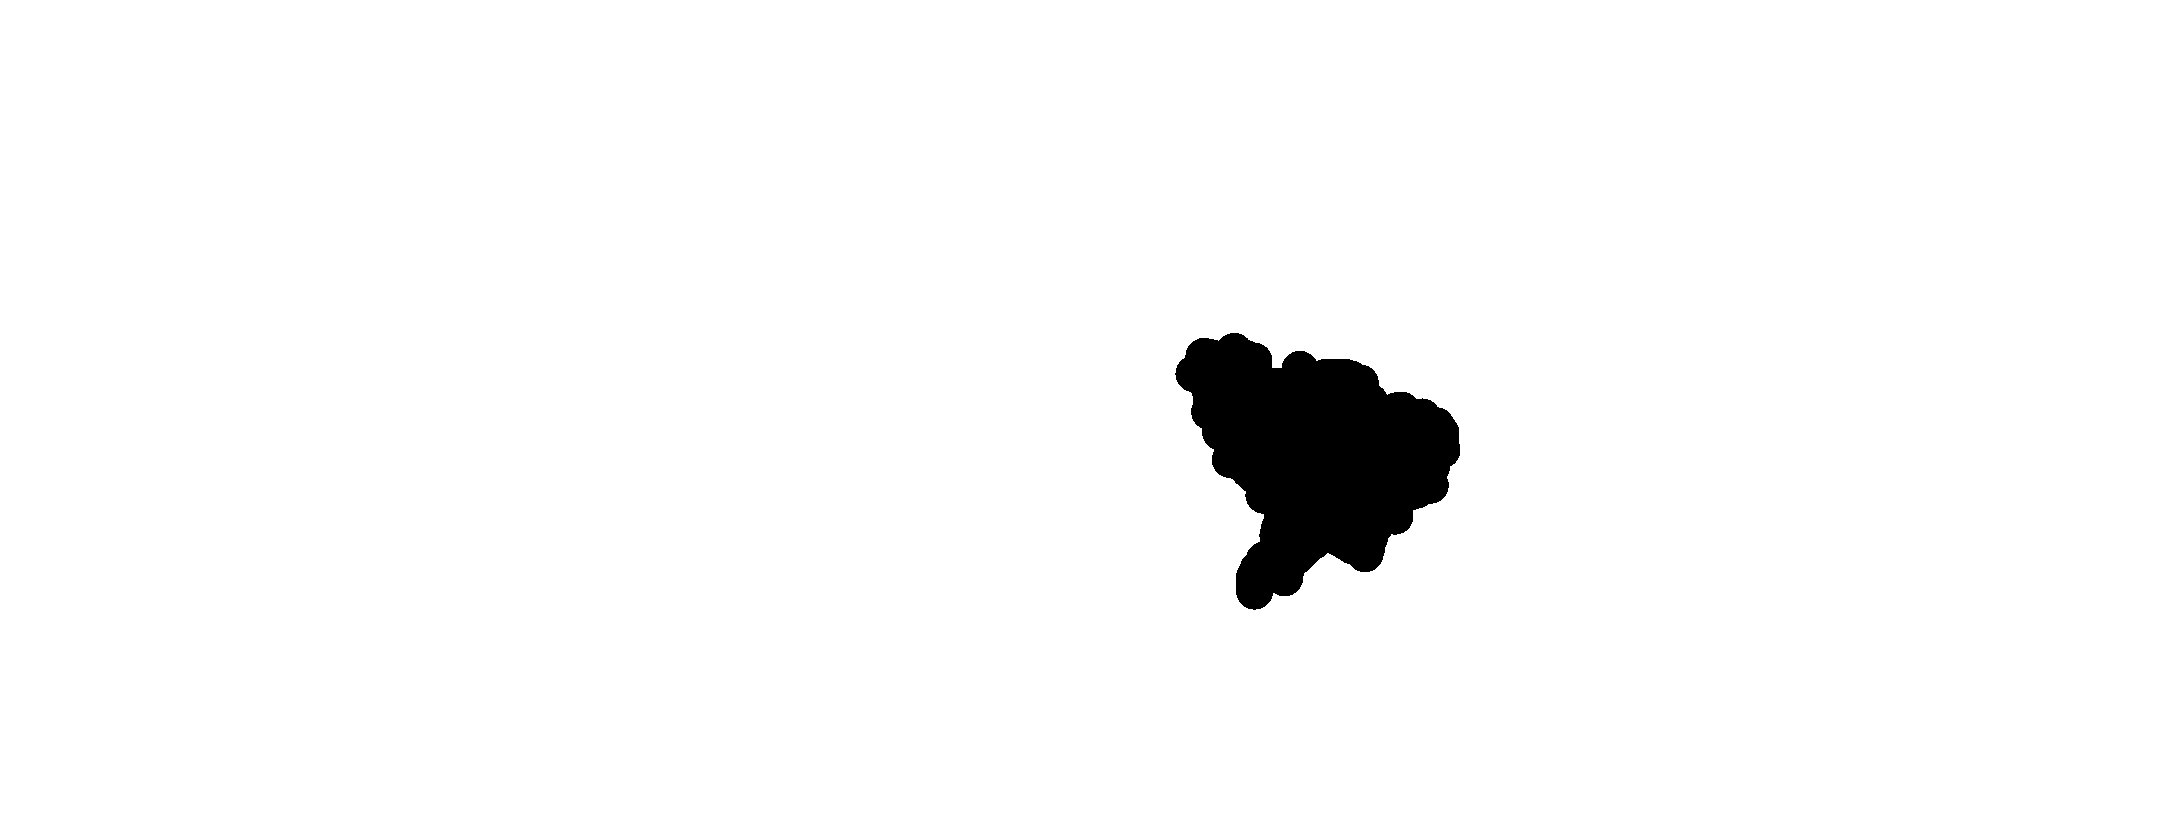
\includegraphics[width=1\linewidth]{Figures/Chapter4/generation-0-melusi}
  \caption*{Initial State}
\end{subfigure}
\begin{subfigure}{.5\textwidth}
  \centering
  
\includegraphics[width=1\linewidth]{Figures/Chapter4/generation-1-melusi}
  \caption*{Generation $t = 1$}
\end{subfigure}
\end{figure}

\begin{figure}[H]
\begin{subfigure}{.5\textwidth}
  \centering
  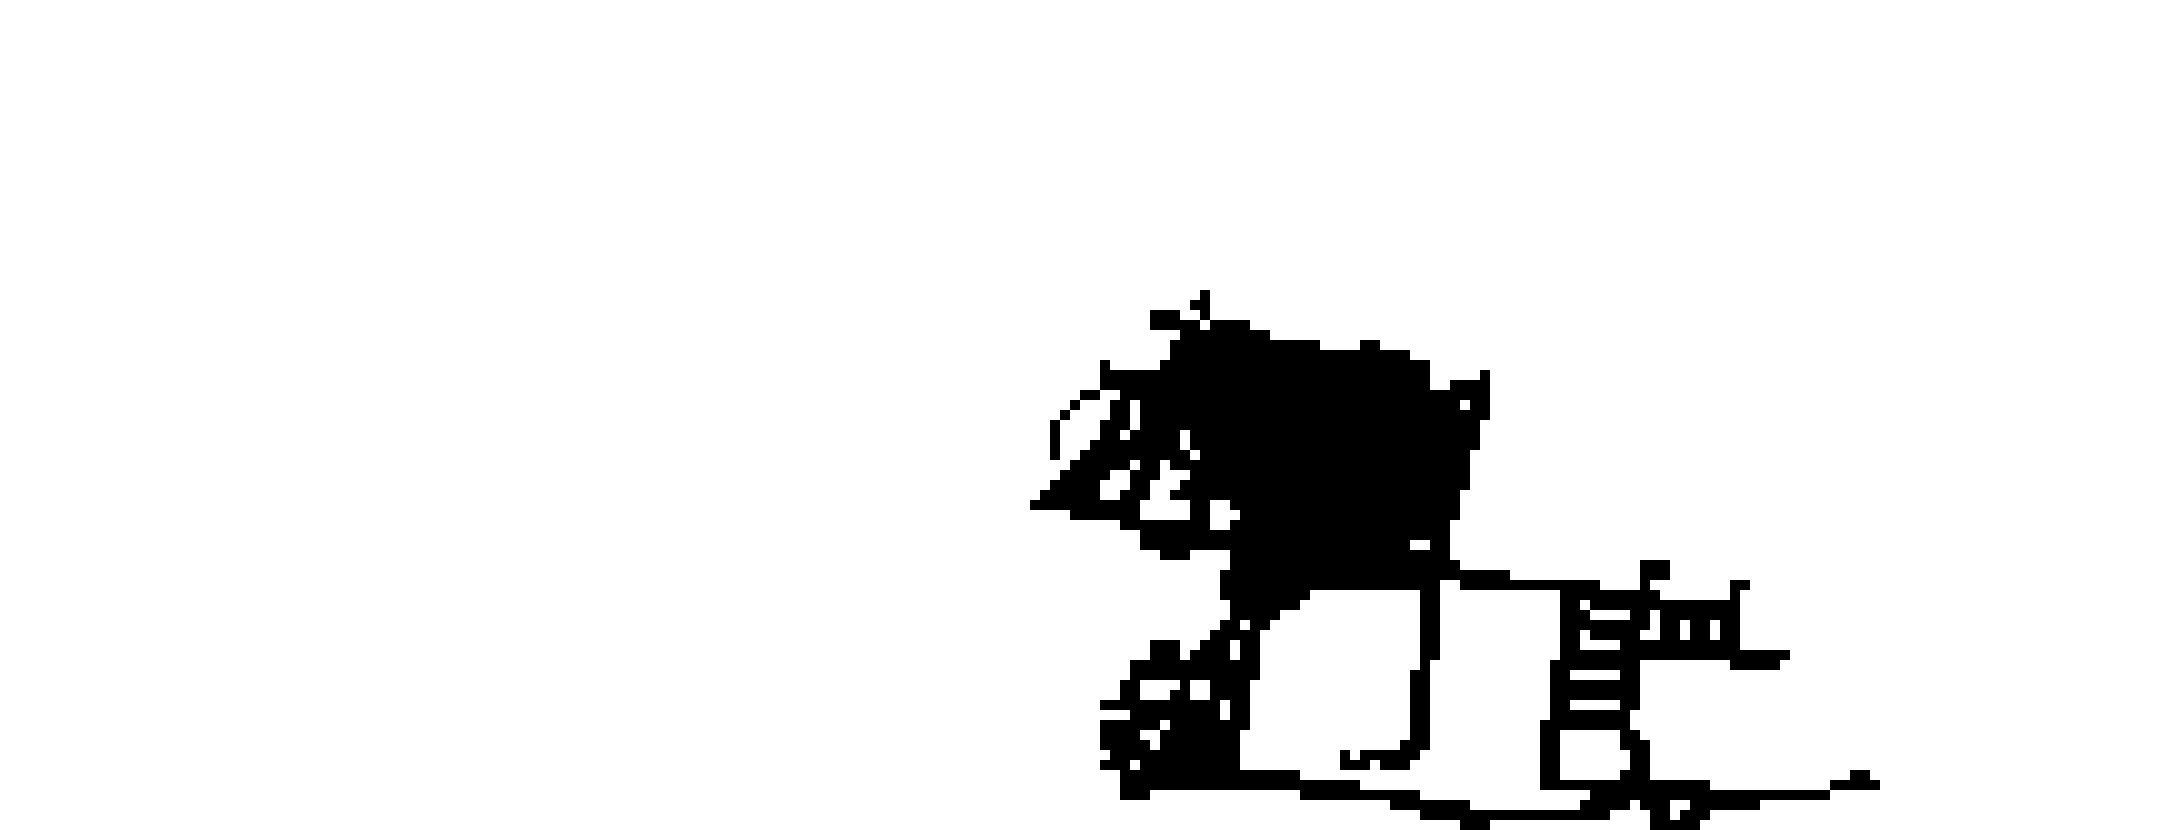
\includegraphics[width=1\linewidth]{Figures/Chapter4/generation-5-melusi}
  \caption*{Generation $t = 5$}
\end{subfigure}
\begin{subfigure}{.5\textwidth}
  \centering
  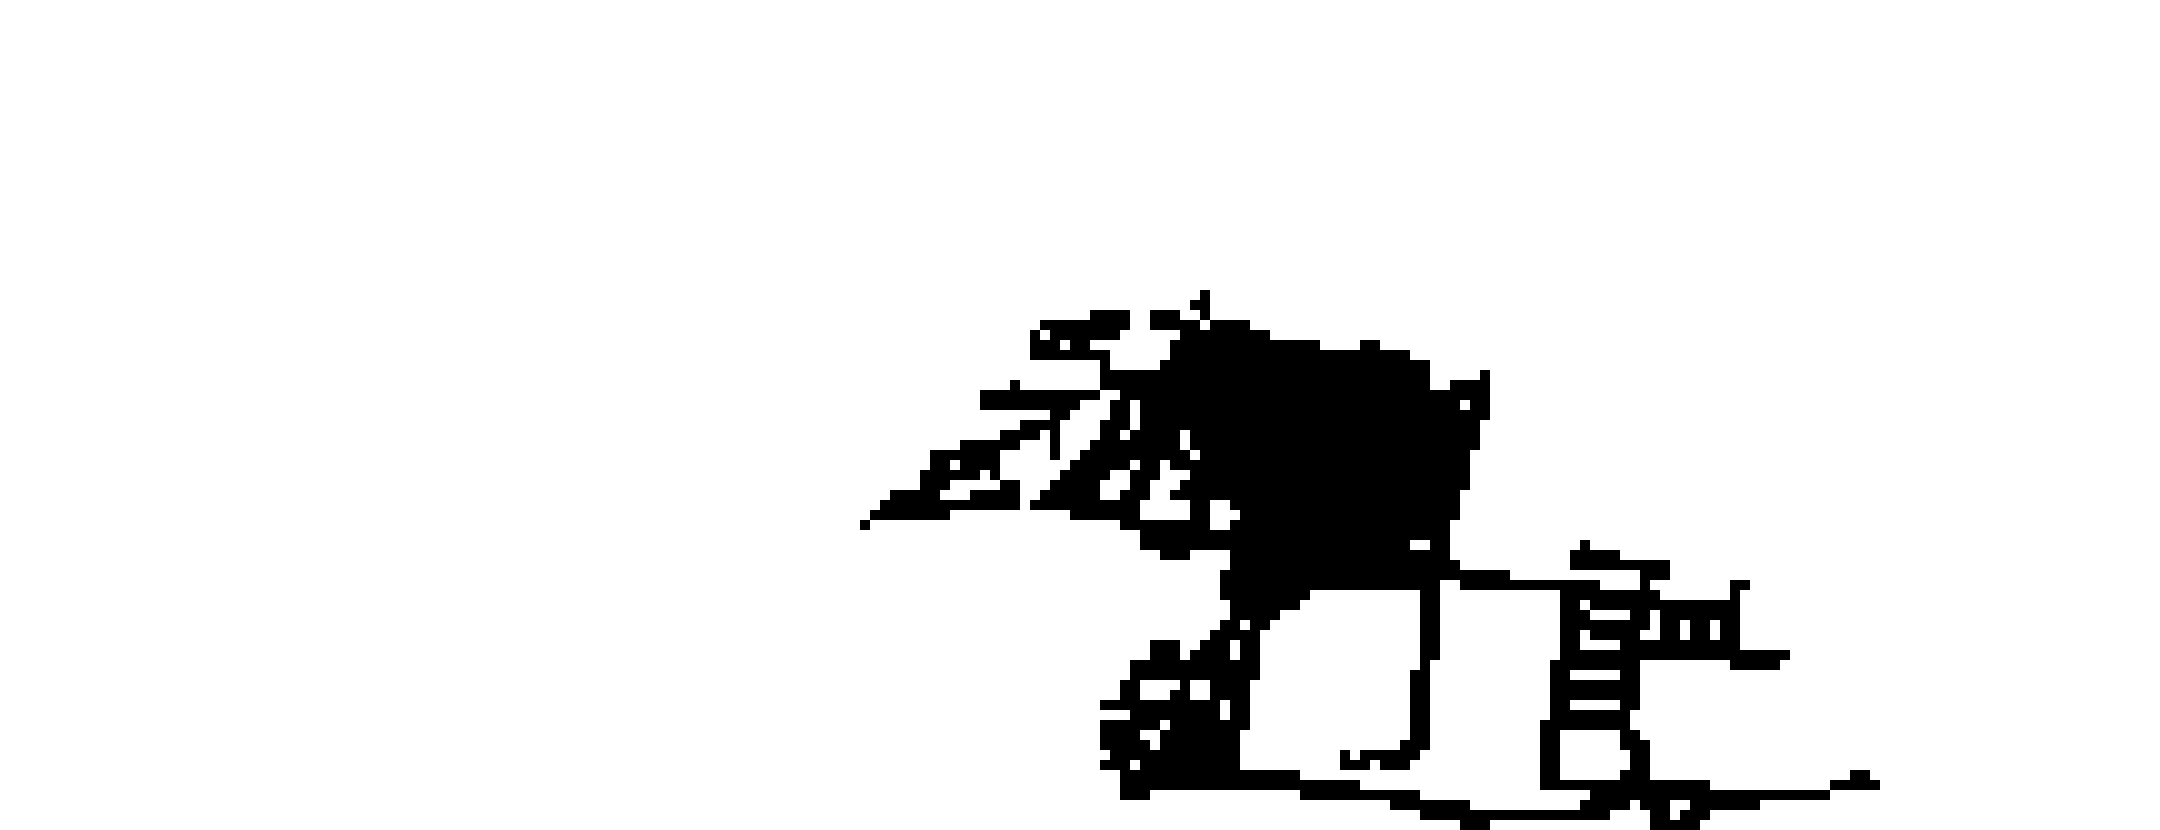
\includegraphics[width=1\linewidth]{Figures/Chapter4/generation-10-melusi}
  \caption*{Generation $t = 10$}
\end{subfigure}
\end{figure}

\begin{figure}[H]
\begin{subfigure}{.5\textwidth}
  \centering
  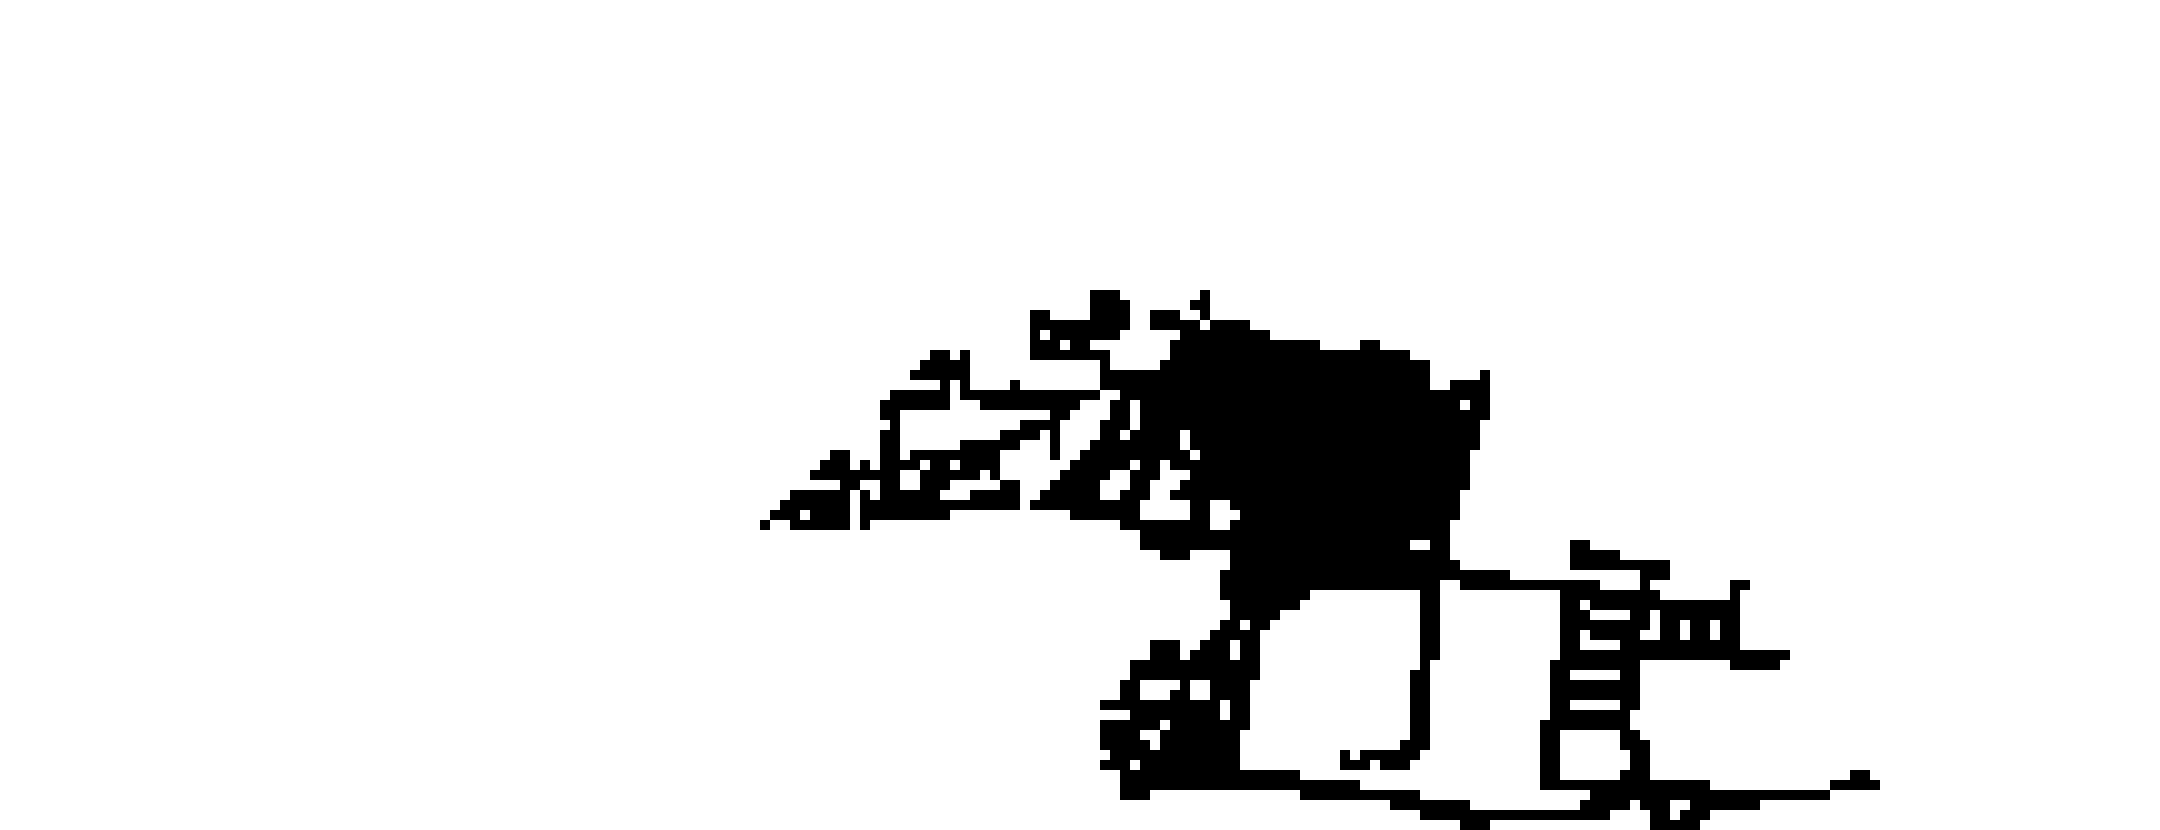
\includegraphics[width=1\linewidth]{Figures/Chapter4/generation-15-melusi}
  \caption*{Generation $t = 15$}
\end{subfigure}
\begin{subfigure}{.5\textwidth}
  \centering
  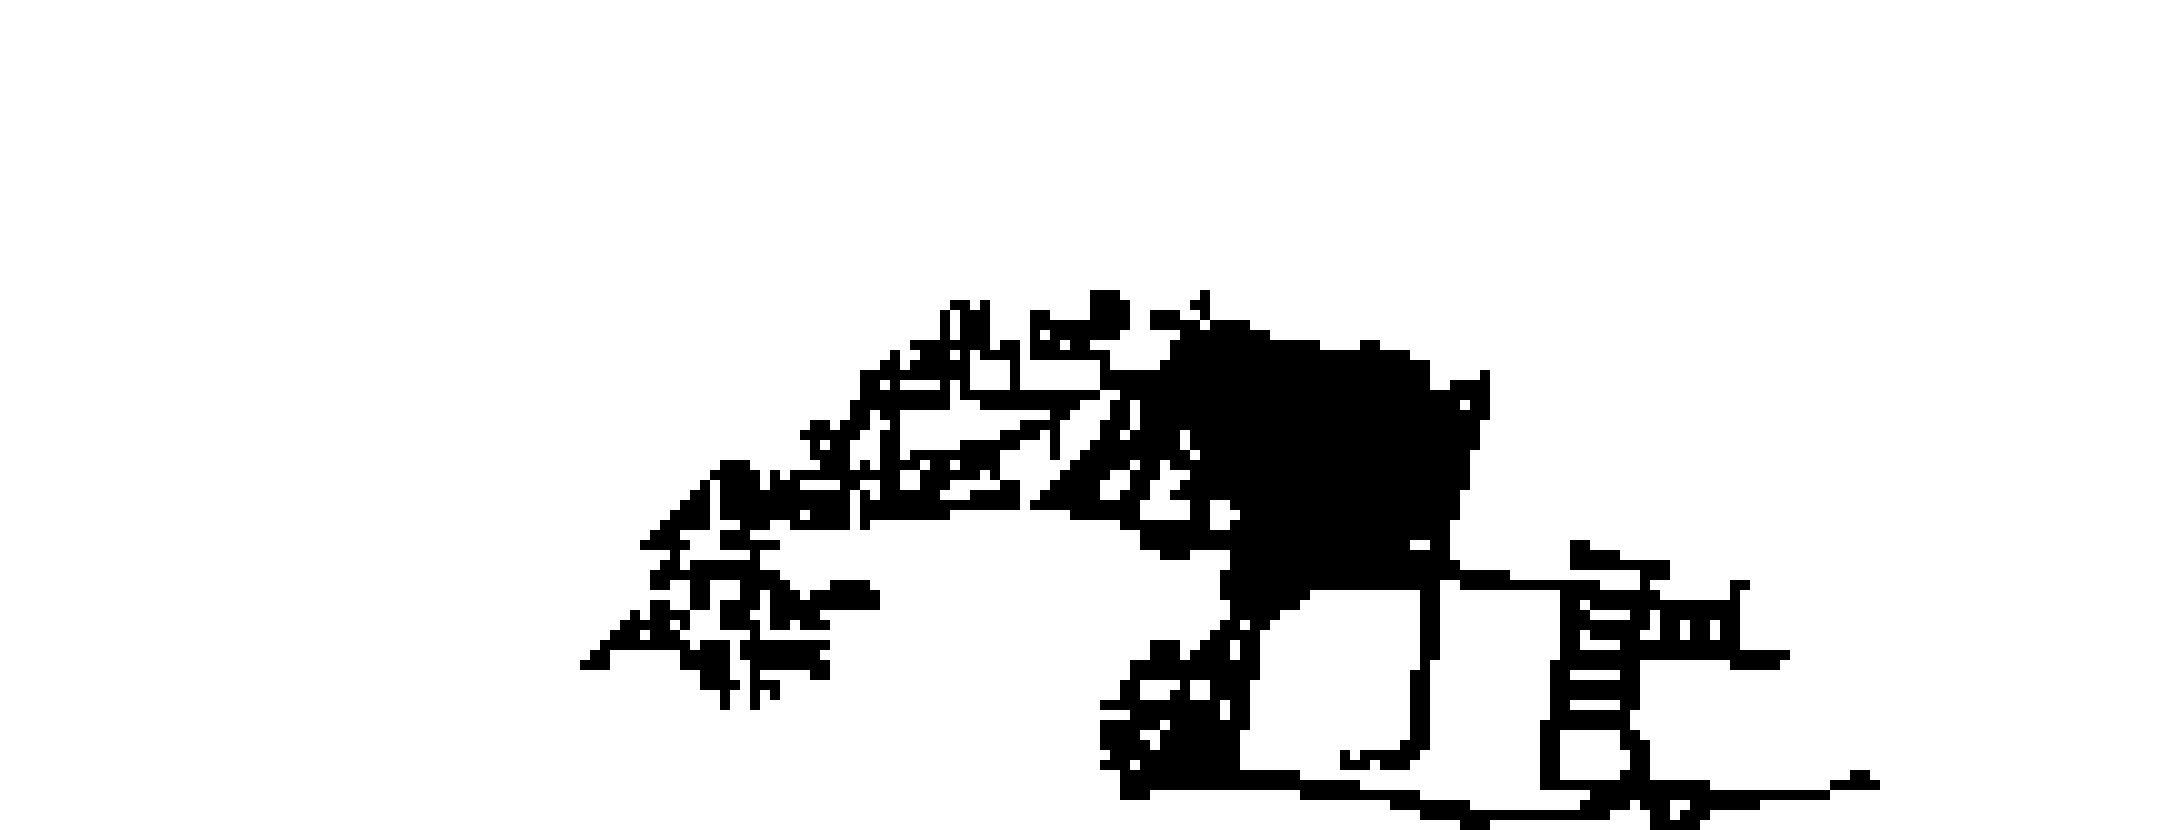
\includegraphics[width=1\linewidth]{Figures/Chapter4/generation-20-melusi}
  \caption*{Generation $t = 20$}
\end{subfigure}
\end{figure}

\begin{figure}[H]
\begin{subfigure}{.5\textwidth}
  \centering
  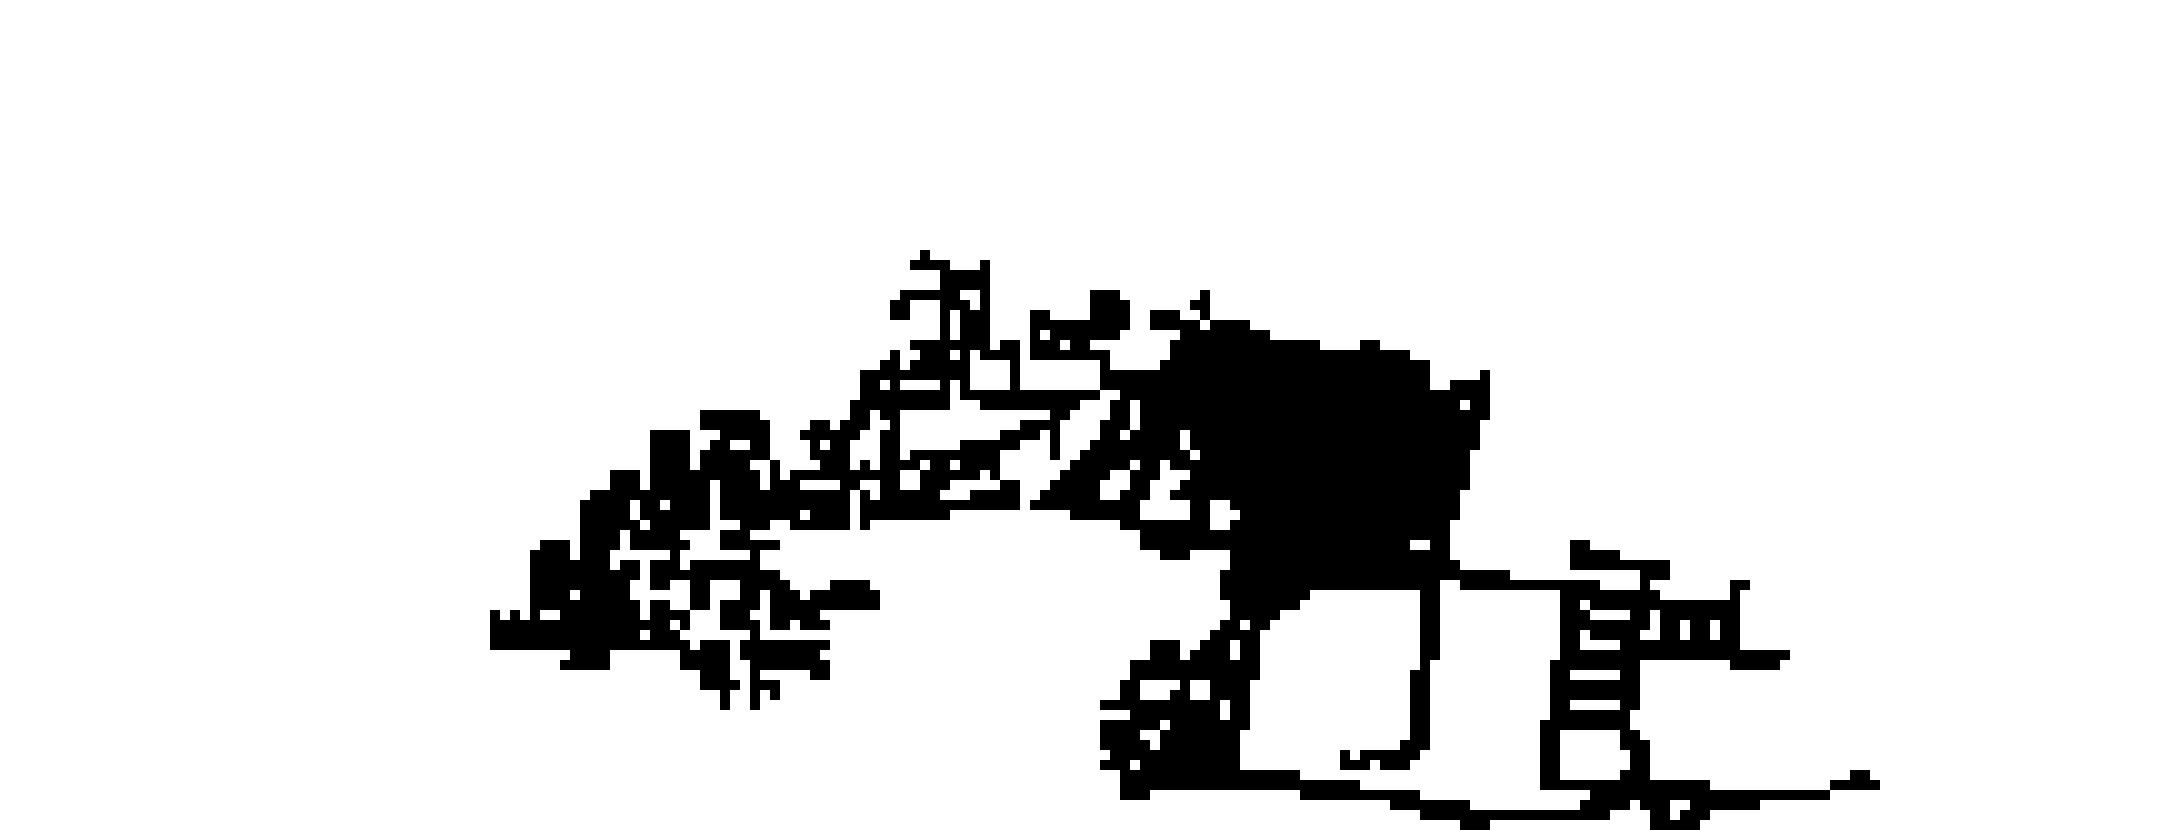
\includegraphics[width=1\linewidth]{Figures/Chapter4/generation-25-melusi}
  \caption*{Generation $t = 25$}
\end{subfigure}
\begin{subfigure}{.5\textwidth}
  \centering
  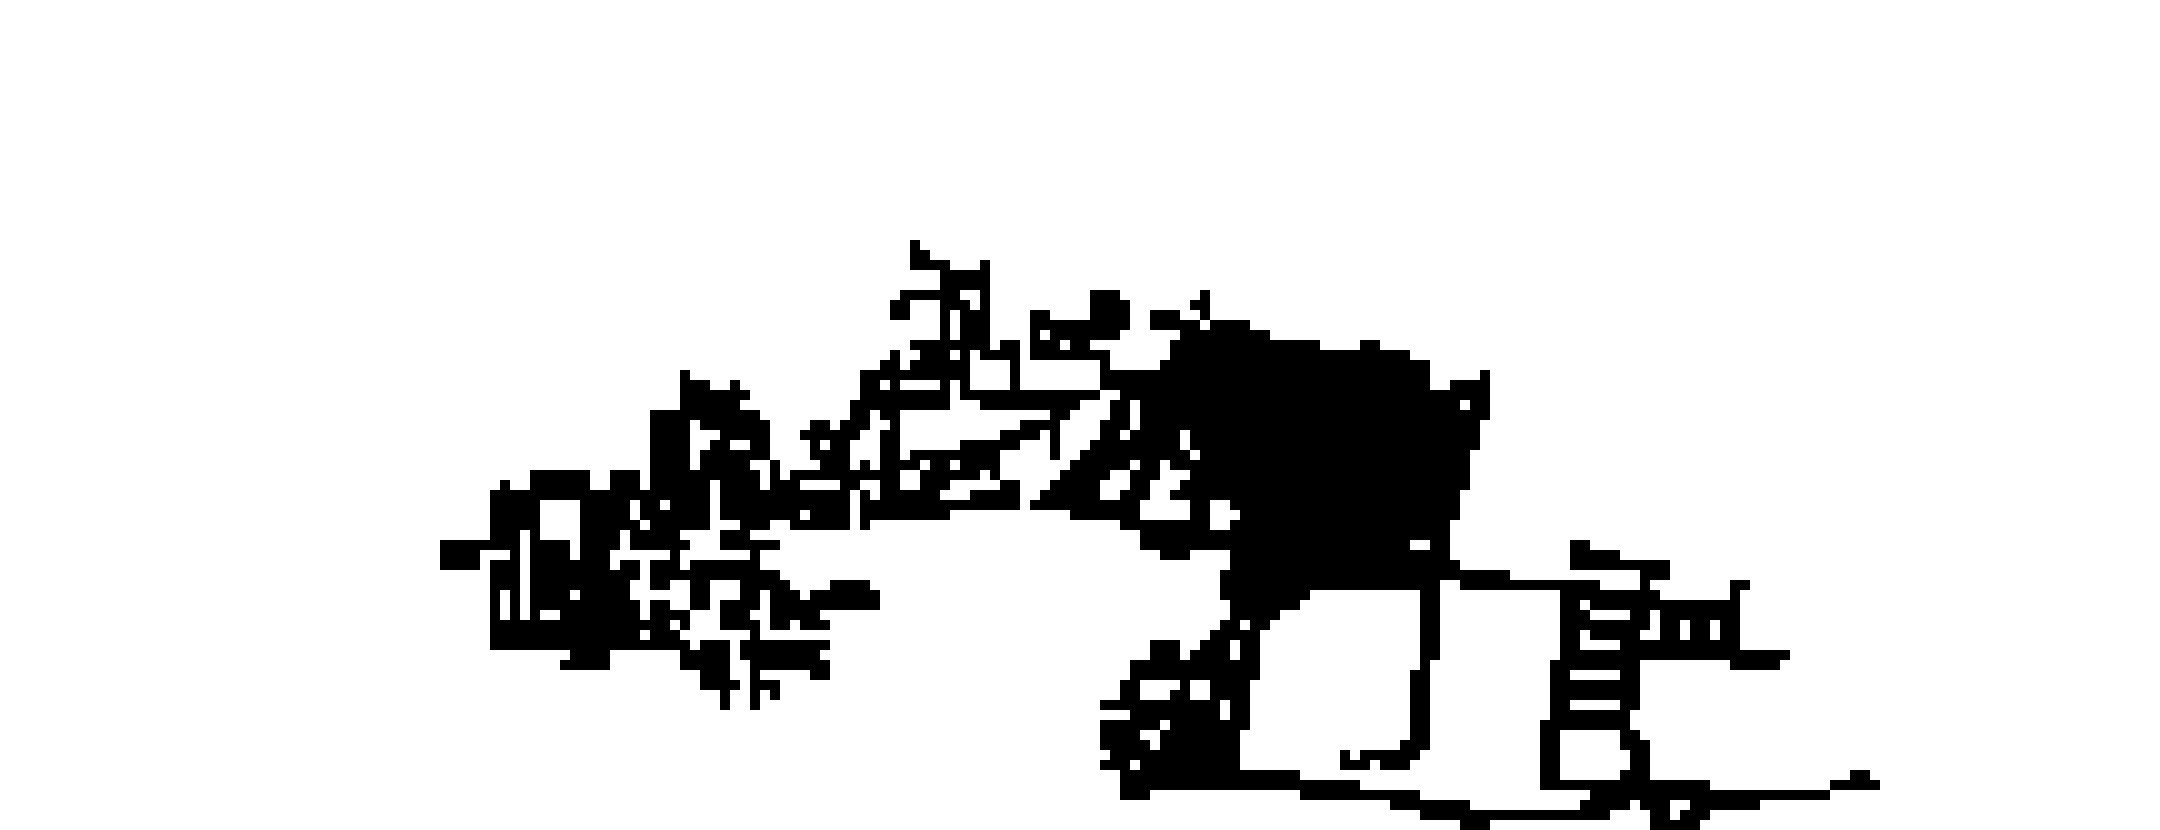
\includegraphics[width=1\linewidth]{Figures/Chapter4/generation-30-melusi}
  \caption*{Generation $t = 30$}
\end{subfigure}
\end{figure}

\begin{figure}[H]
\begin{subfigure}{.5\textwidth}
  \centering
  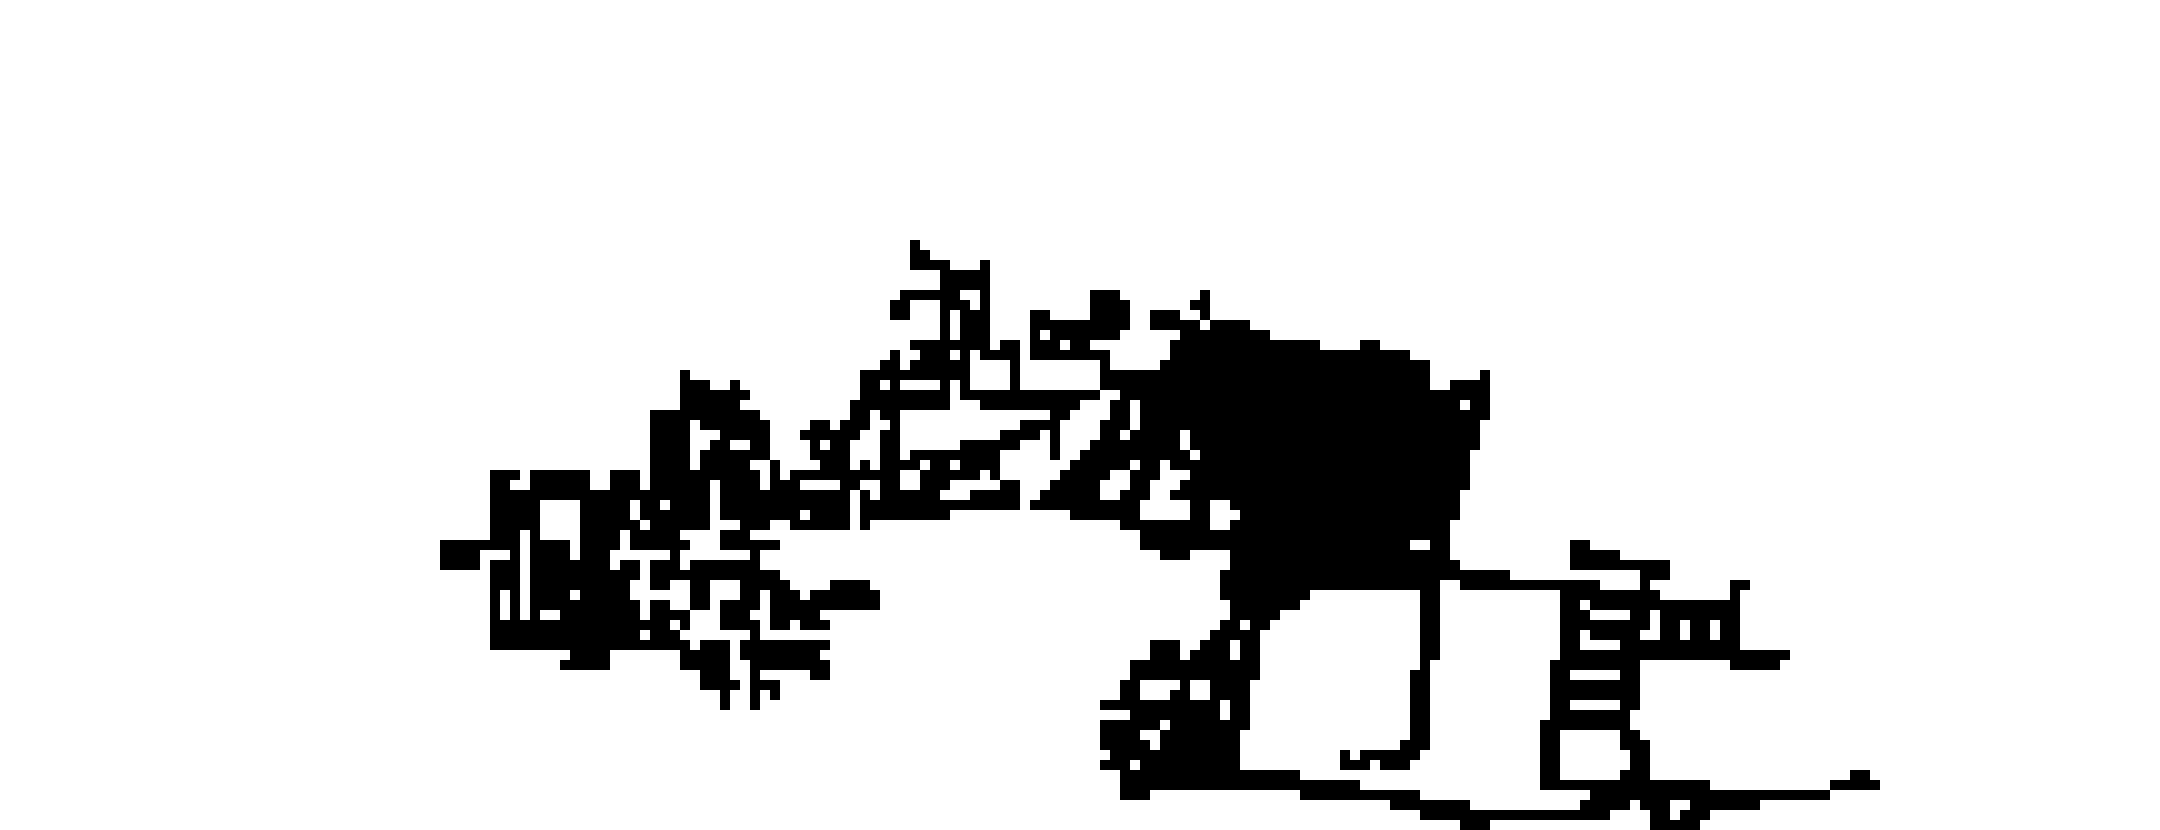
\includegraphics[width=1\linewidth]{Figures/Chapter4/generation-35-melusi}
  \caption*{Generation $t = 35$}
\end{subfigure}
\begin{subfigure}{.5\textwidth}
  \centering
  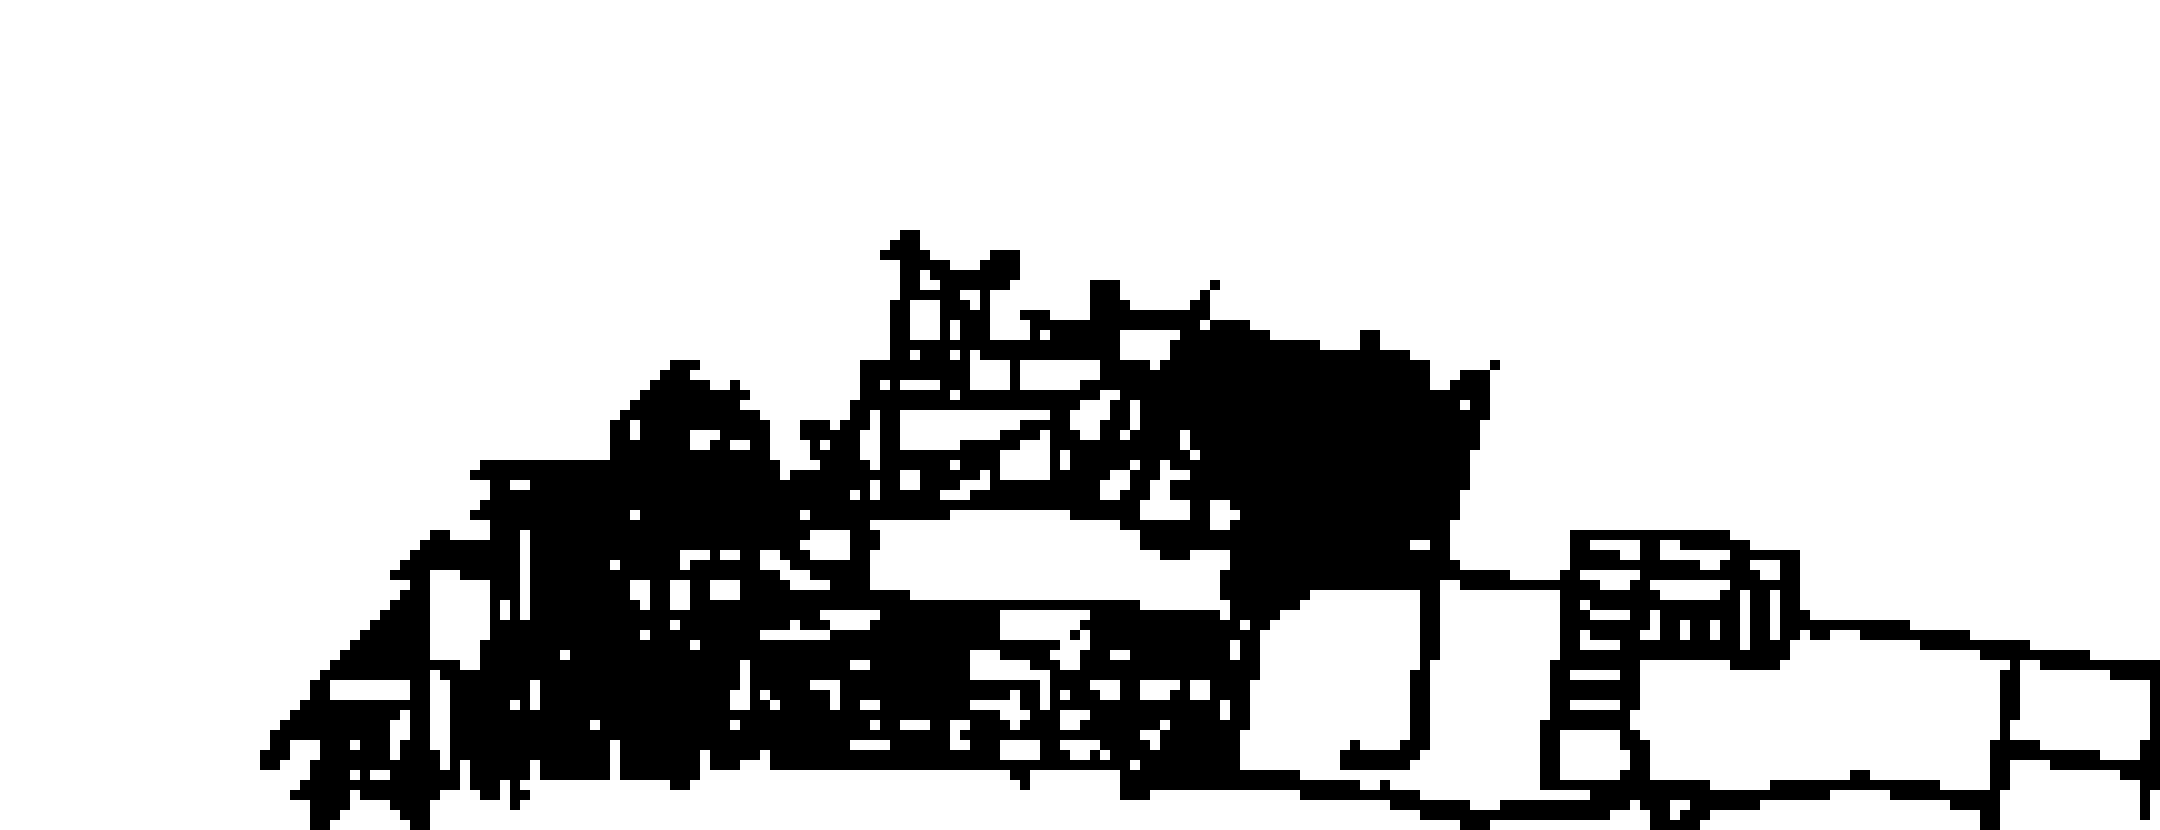
\includegraphics[width=1\linewidth]{Figures/Chapter4/generation-40-melusi}
  \caption*{Generation $t = 40$}
\end{subfigure}
\end{figure}

\begin{figure}[H]
\begin{subfigure}{.5\textwidth}
  \centering
  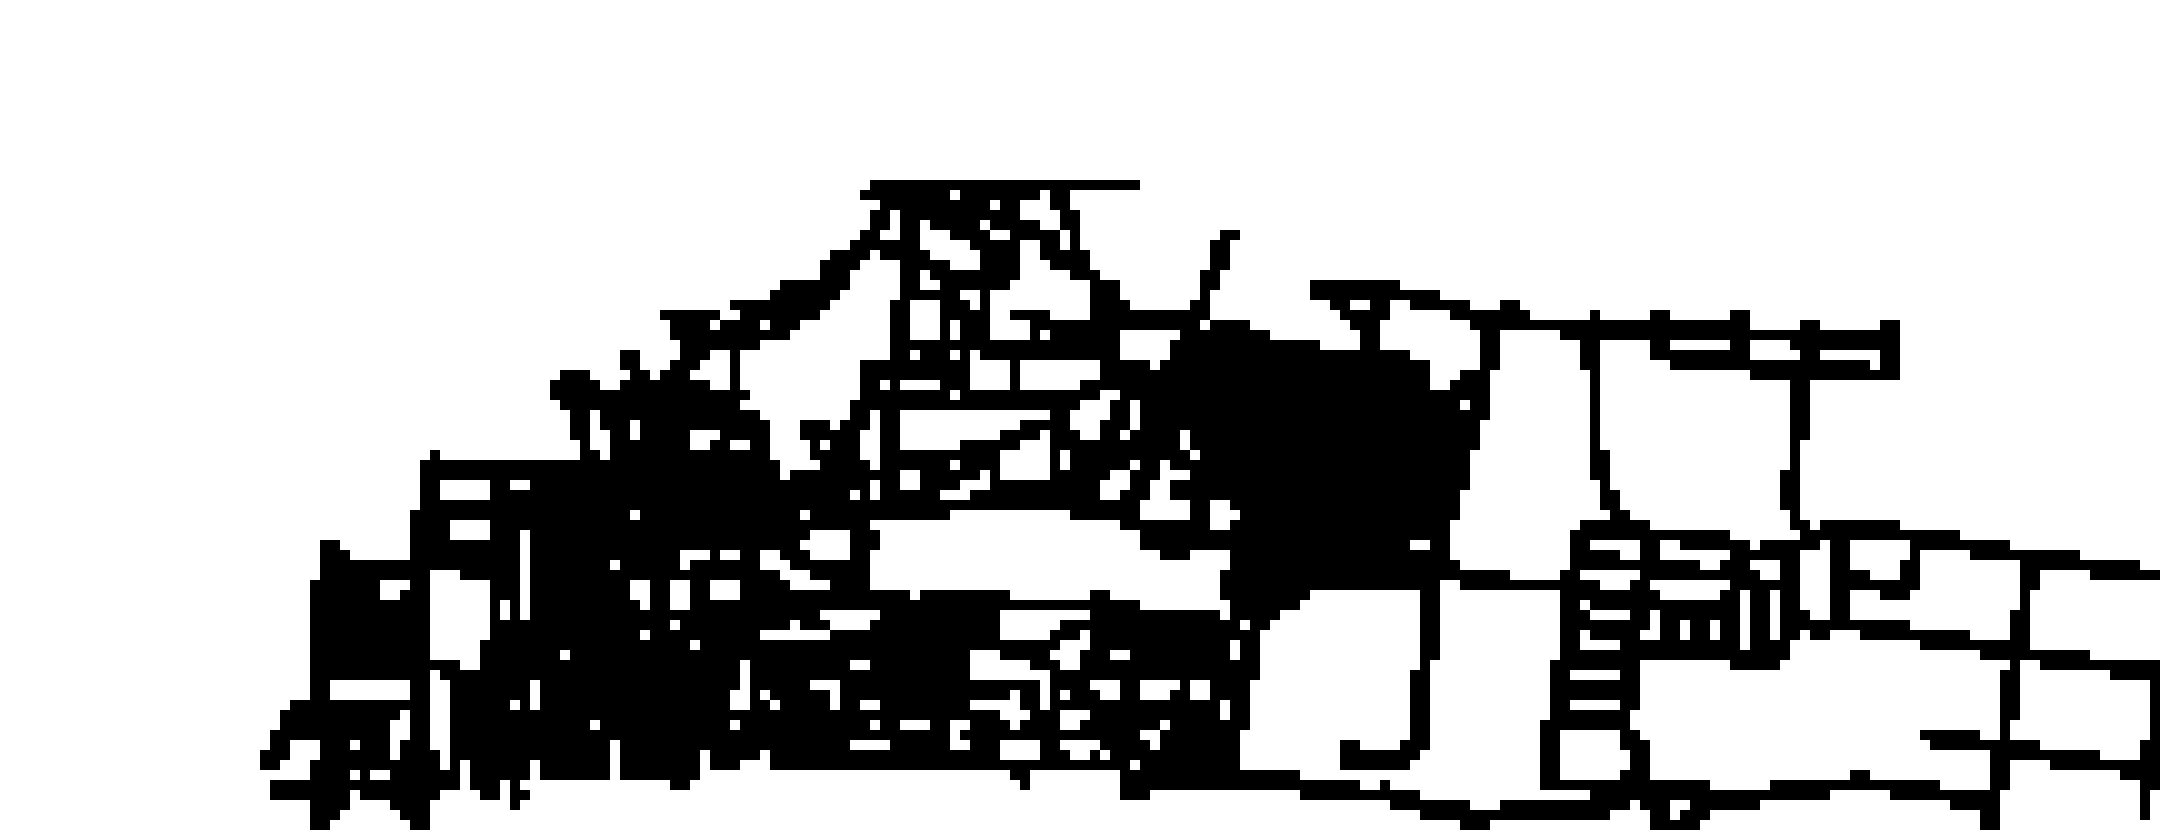
\includegraphics[width=1\linewidth]{Figures/Chapter4/generation-45-melusi}
  \caption{Generation $t = 45$}
\end{subfigure}
\begin{subfigure}{.5\textwidth}
  \centering
  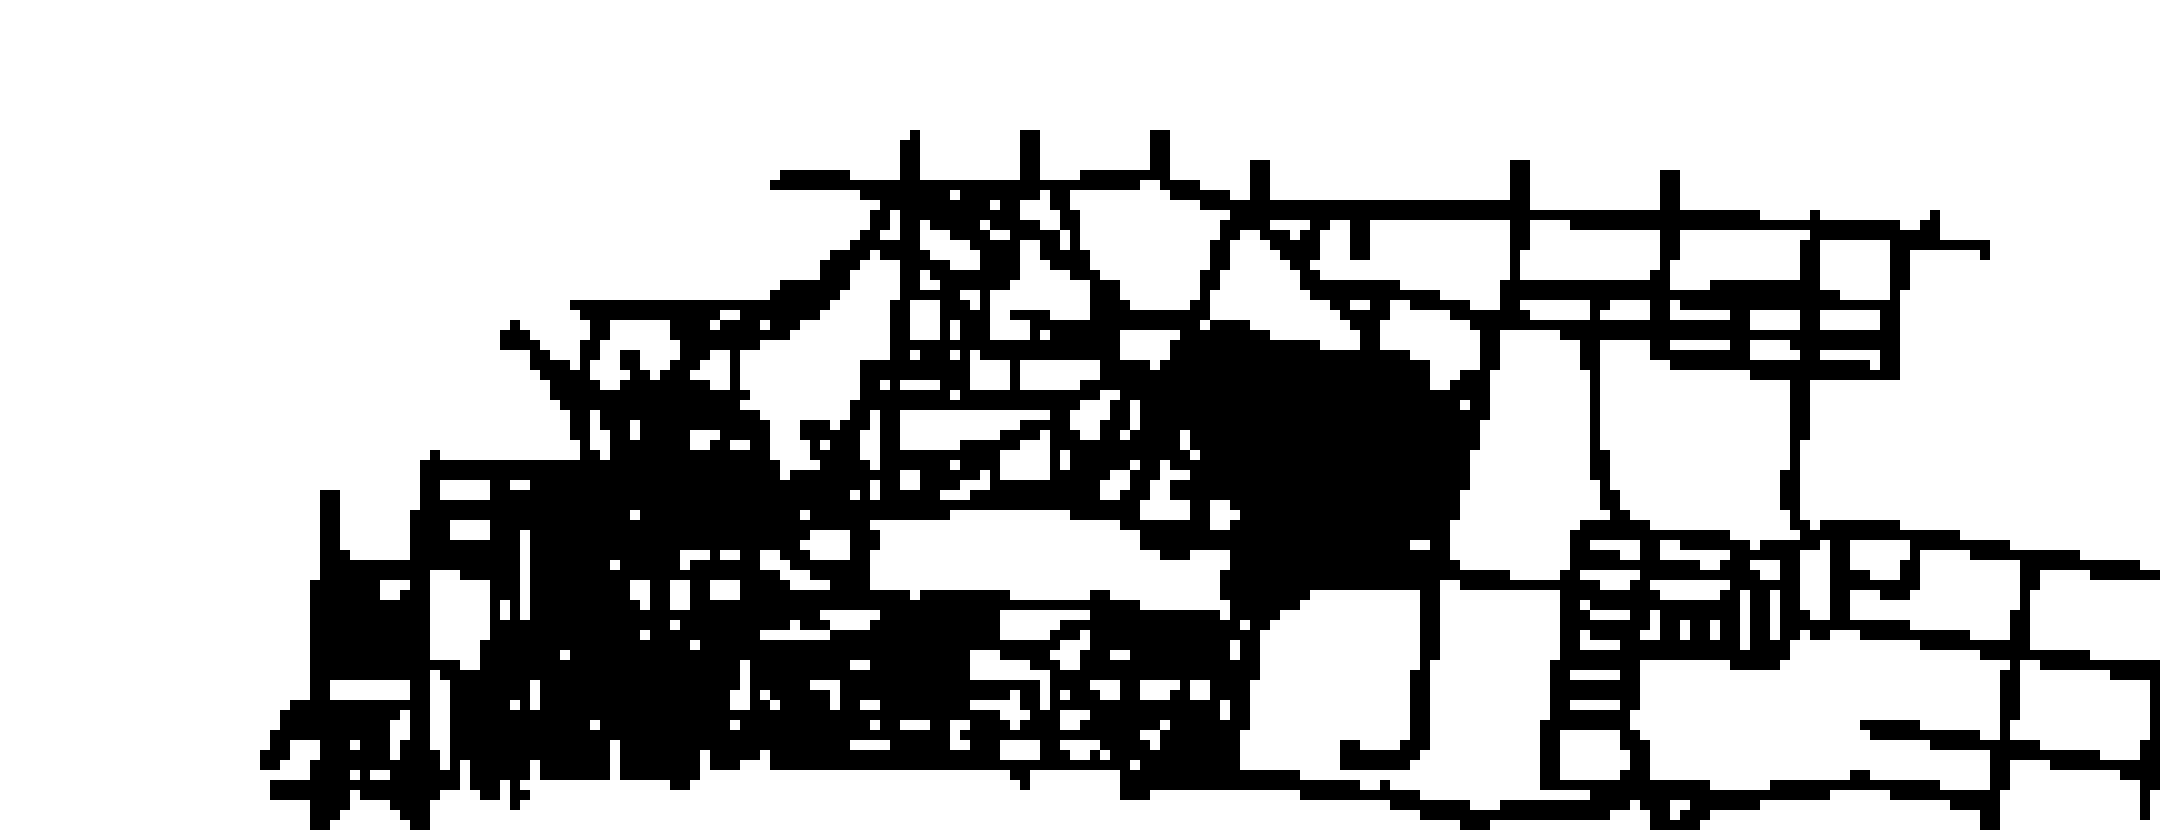
\includegraphics[width=1\linewidth]{Figures/Chapter4/generation-50-melusi}
  \caption{Generation $t = 50$}
\end{subfigure}
\caption{Simulated Growth for different periods of the 50 Generations}
\label{fig:gen50}
\end{figure}
\begin{center}
Source: Own Creation (2021)
\end{center}

\begin{figure}[H]
\centering
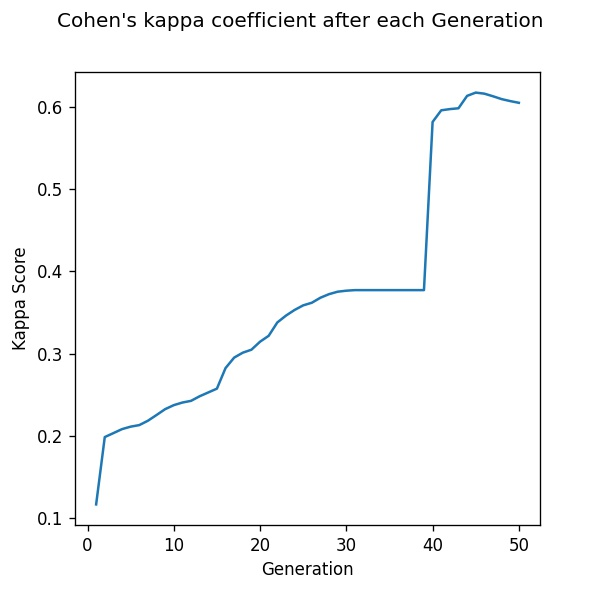
\includegraphics[scale=0.7]{Figures/Chapter4/scoresFigure}
\caption{Kappa coefficient for each generation simulated}
\end{figure}

\begin{figure}[H]
\centering
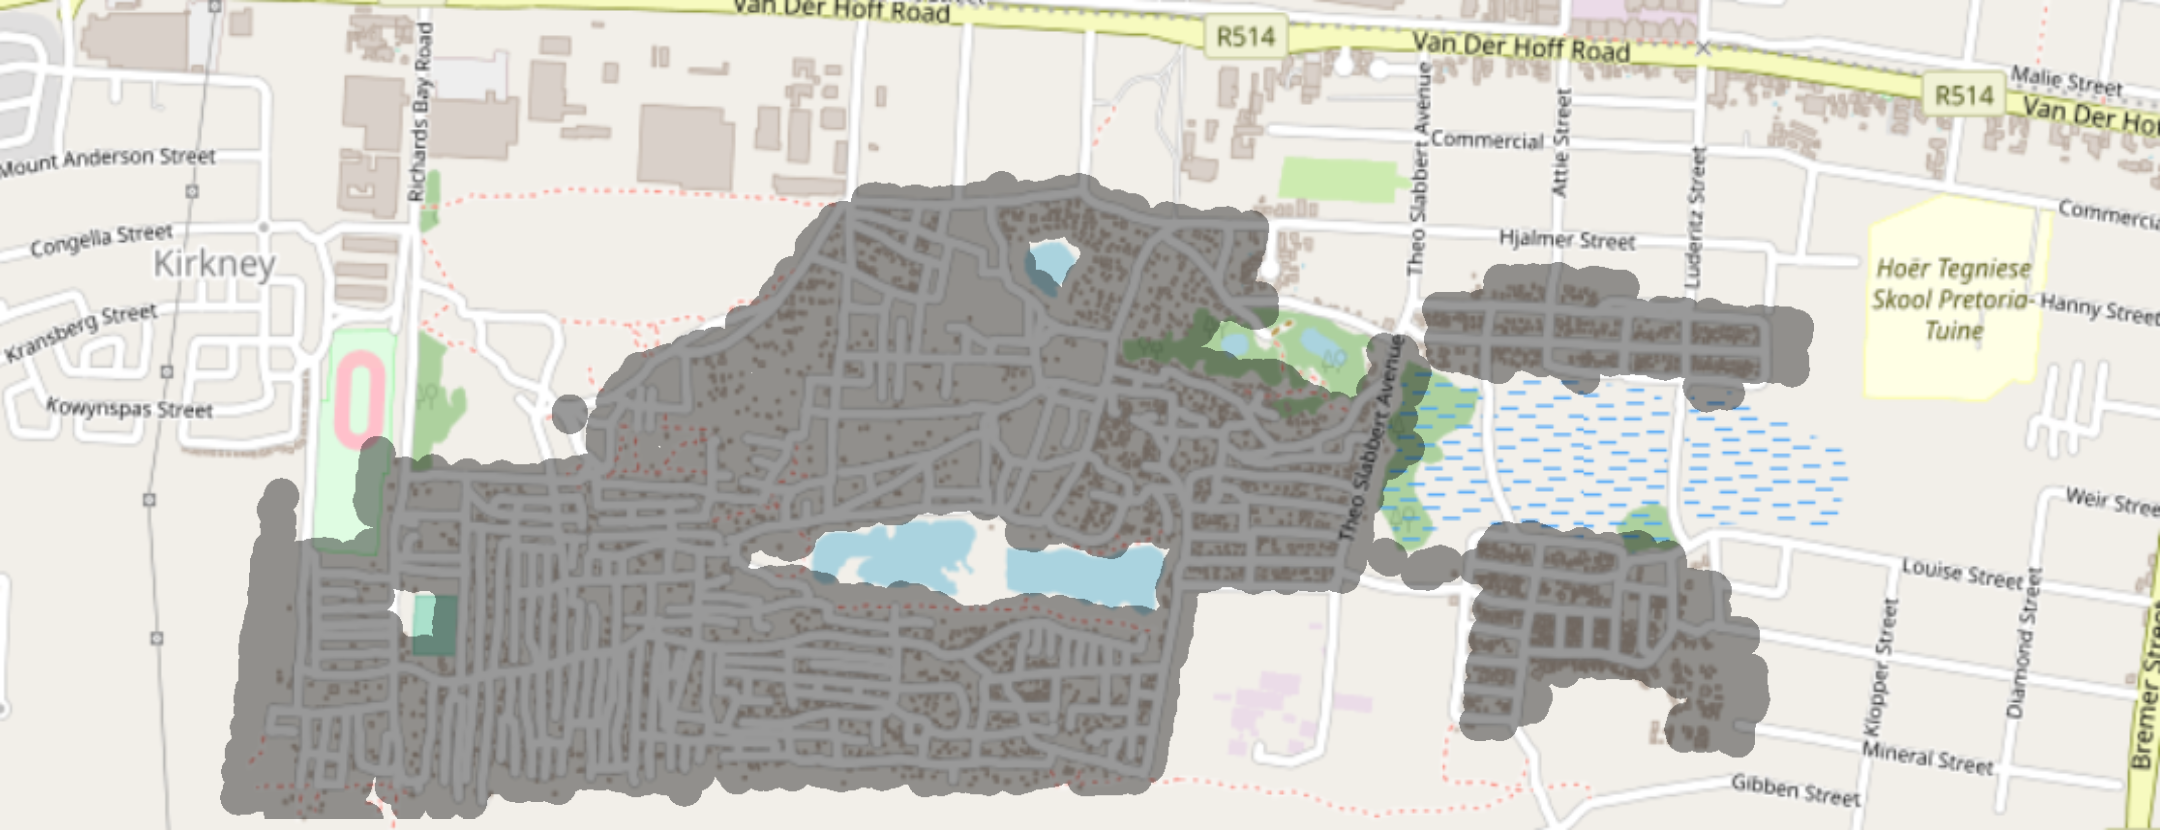
\includegraphics[scale=0.3,angle=90]{Figures/Chapter4/Actual}
\caption{Existing Building Based Land Usage on a Map}
\end{figure}

\begin{figure}[H]
\centering
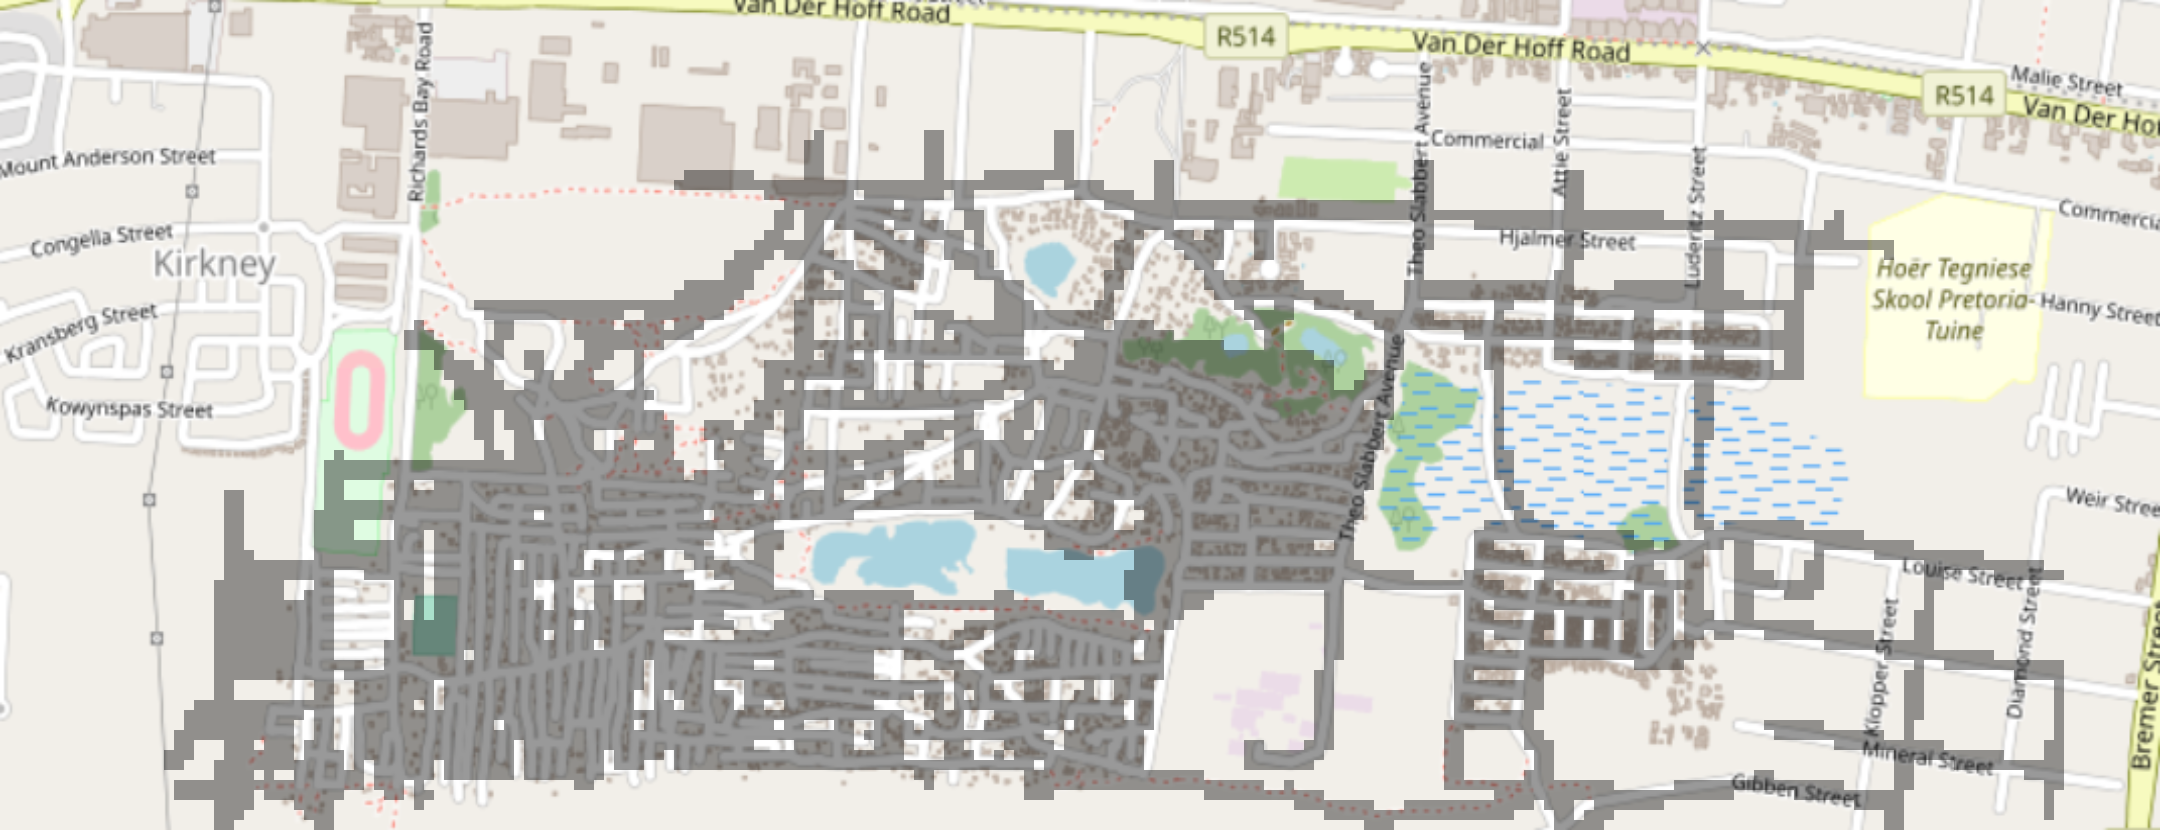
\includegraphics[scale=0.3,angle=90]{Figures/Chapter4/Simulated}
\caption{Simulated Growth of Building Based Land Usage on a Map}
\end{figure}

\begin{table}[H]
\setlength{\tabcolsep}{12pt}
\renewcommand{\arraystretch}{1.1}
    \caption{Accuracy results for each time step}
    \begin{minipage}{.5\linewidth}
      %\caption{}
            \begin{tabular}{@{}cl@{}}
            \toprule
            Generation & $\kappa$ coefficient \\ \midrule
            1 &  0.11625181498059378 \\
2 &  0.19824922121107136 \\
3 &  0.20306283544626080 \\
4 &  0.20793481429046645 \\
5 &  0.21093437785824343 \\
6 &  0.21283046681369622 \\
7 &  0.21812986043325577 \\
8 &  0.22511088417746883 \\
9 &  0.23225494066337948 \\
10 & 0.23712807908806854 \\
11 & 0.24030784142599682 \\
12 & 0.24236259441785502 \\
13 & 0.24795555301338124 \\
14 & 0.25260419032659376 \\
15 & 0.25724181362747820 \\
16 & 0.28227924369204370 \\
17 & 0.29504157655474317 \\
18 & 0.30102906854032363 \\
19 & 0.30464884852311600 \\
20 & 0.31438848428890310 \\
21 & 0.32157142237699610 \\
22 & 0.33780443805206917 \\
23 & 0.34613948926327110 \\
24 & 0.35302831352863406 \\
25 & 0.35866215860009740 \\ \bottomrule
        \end{tabular}
    \end{minipage}%
    \begin{minipage}{.5\linewidth}
        %\caption{}
        \begin{tabular}{@{}cl@{}}
          \toprule
          Generation & $\kappa$ coefficient \\ \midrule
          26 & 0.36182388889416850 \\
          27 & 0.36795669505675166 \\ 
          28 & 0.37232518280926630 \\
          29 & 0.37529002091648256 \\
          30 & 0.37650949057057026 \\
          31 & 0.37720597829276714 \\
          32 & 0.37720597829276714 \\
          33 & 0.37720597829276714 \\
          34 & 0.37720597829276714 \\
          35 & 0.37720597829276714 \\
          36 & 0.37720597829276714 \\
          37 & 0.37720597829276714 \\
          38 & 0.37720597829276714 \\
          39 & 0.37720597829276714 \\
          40 & 0.58197245681417580 \\
          41 & 0.59617325191136350 \\
          42 & 0.59765374964576660 \\
          43 & 0.59865025952753870 \\
          44 & 0.61375538510117190 \\
          \textbf{45} & \textbf{0.61775529641454560} \\
          46 & 0.61644571800015240 \\
          47 & 0.61328585200053230 \\
          48 & 0.60982488474318350 \\
          49 & 0.60740162003478520 \\
          50 & 0.60532388693353810 \\ \bottomrule
      \end{tabular}
      %\vspace*{0.8in}
    \end{minipage}
\end{table}